For precision measurement of the physics processes at the LHC, an accurate
description of the \gls{pdf} is important. The parton distribution functions are
non-perturbative and extracted from global fit to hard-scatter data. Two kind of
\glspl{pdf} are considered:
\begin{itemize}
\item Intra-\gls{pdf} uncertainty: This is the uncertainty within a specific \gls{pdf}
  set.
\item Inter-\gls{pdf} uncertainty: This is the uncertainty when a certain
  \gls{pdf} is replaced with another.
\end{itemize}
Three different groups provide equally precise parton distribution functions
making it arbitrary to use one over the others to generate the signal MC
samples. For this reason the recommendation of the PDF4LHC~\cite{PDF4LHC} group
for a correct estimation of the \gls{pdf} uncertainty is to combine the
uncertainties from all three groups and thus the CT10~\cite{CT10}, the
NNPDF~\cite{NNPDF} and the MMHT~\cite{MMHT} \gls{pdf} sets have been used.

The \gls{mc} signal samples for the \gls{susy} compressed models are generated
using the NNPDF set, in principle in order to evaluate the \gls{pdf}
uncertainties for CT10 and MMHT it would be necessary to re-generate the signal
samples using these \gls{pdf} sets. It is common practice to instead re-weight
each event in the original sample to the value it would have if it were
generated using an alternate PDF set. This is done using the
LHAPDF~\cite{LHAPDF} tool.
% The weight is given by:
% \begin{equation}
%   \label{eq:118}
%   w = \frac{\mathrm{PDF}(x_1, f_1, Q) \cdot \mathrm{PDF}(x_2, f_2, Q)}
%   {\mathrm{PDF}_0(x_1, f_1, Q) \cdot \mathrm{PDF}_0(x_2, f_2, Q)}
% \end{equation}
% where $\mathrm{PDF}$ is the alternate \gls{pdf} and $\mathrm{PDF}_0$ is the
% \gls{pdf} used to generate the samples.

The CT10 and the MMHT sets provide error sets to estimate the intra-\gls{pdf}
uncertainty. The idea is that each \gls{pdf} has a number of uncorrelated
parameters that can be varied independently by $\pm 1\sigma$ and a new \gls{pdf}
can be calculated. This procedure is then repeated for each parameter in the
\gls{pdf} set resulting in a set of \glspl{pdf}. This procedure is also done
using the LHAPDF tool. The Hessian~\cite{Hessian} method is then used to
estimate the uncertainty on the sets of \glspl{pdf}.

For CT10 the symmetric Hessian method with 52 error sets is used where the
uncertainty is given by:
\begin{equation}
  \label{eq:119}
  \delta X = \sqrt{\sum_{k = 1}^{n_\mathrm{err}} \left(X^{(k)} -
      X^{(0)} \right)^2}
\end{equation}
where $X^{(0)}$ is the number of events using the best \gls{pdf} fit and
$X^{(k)}$ is the number of events using the \gls{pdf} calculated varying the
$k$-th parameter.

For MMHT the asymmetric Hessian method with 50 error sets is used and the
uncertainty is given by:
\begin{align}
  \label{eq:120}
  \delta x^{\mathrm{up}} & = \sqrt{\sum_{k = 1}^{n_\mathrm{err}/2}
                           \mathrm{max}(0, X_{2k} - X_0, X_{2k - 1} - X_0)^2} \\
  \delta x^{\mathrm{dw}} & = \sqrt{\sum_{k = 1}^{n_\mathrm{err}/2}
                           \mathrm{max}(0, X_0 - X_{2k}, X_0 - X_{2k - 1})^2}
\end{align}
where $X_0$ is the number of events obtained with the best fit and $X_{2k}
(X_{2k -1})$ is the number of events calculated with the $2k$-th ($2k -1$-th)
parameter variation.

The NNPDF group provides an ensemble of 100 different and equally good
\glspl{pdf}. The one used to generate the signal samples (the \emph{nominal}) is
then obtained calculating the mean of the provided set while the associated
intra-\gls{pdf} systematic uncertainty is given by the standard deviation.

The \gls{pdf} systematic uncertainty is decomposed in:
\begin{itemize}
\item An uncertainty $\Delta \sigma$ on the overall normalisation or cross
  section, given by the variation of the total number of signal events,
\item An uncertainty $\Delta A$ on the signal acceptance, which is defined by
  the ratio of number of signal events in a particular bin of the signal region,
  divided by the total number of signal events.
\end{itemize}
This decomposition is done since the \gls{atlas} standard is to depict the
uncertainty on the overall normalization as an uncertainty on the expected
limits, while the uncertainty on acceptance is to be incorporated in the
uncertainty on the observed limits. \cref{fig:pdf_syst} presents an example of
the results in terms of weighted signal yields for the acceptance as a function
of the \gls{pdf} family and its uncertainty source. It shows the inter-\gls{pdf}
and intra-\gls{pdf} uncertainties of the three families. The final \gls{pdf}
uncertainty is the envelope that contains the error bands of the three families.
\begin{figure}[!h]
\centering
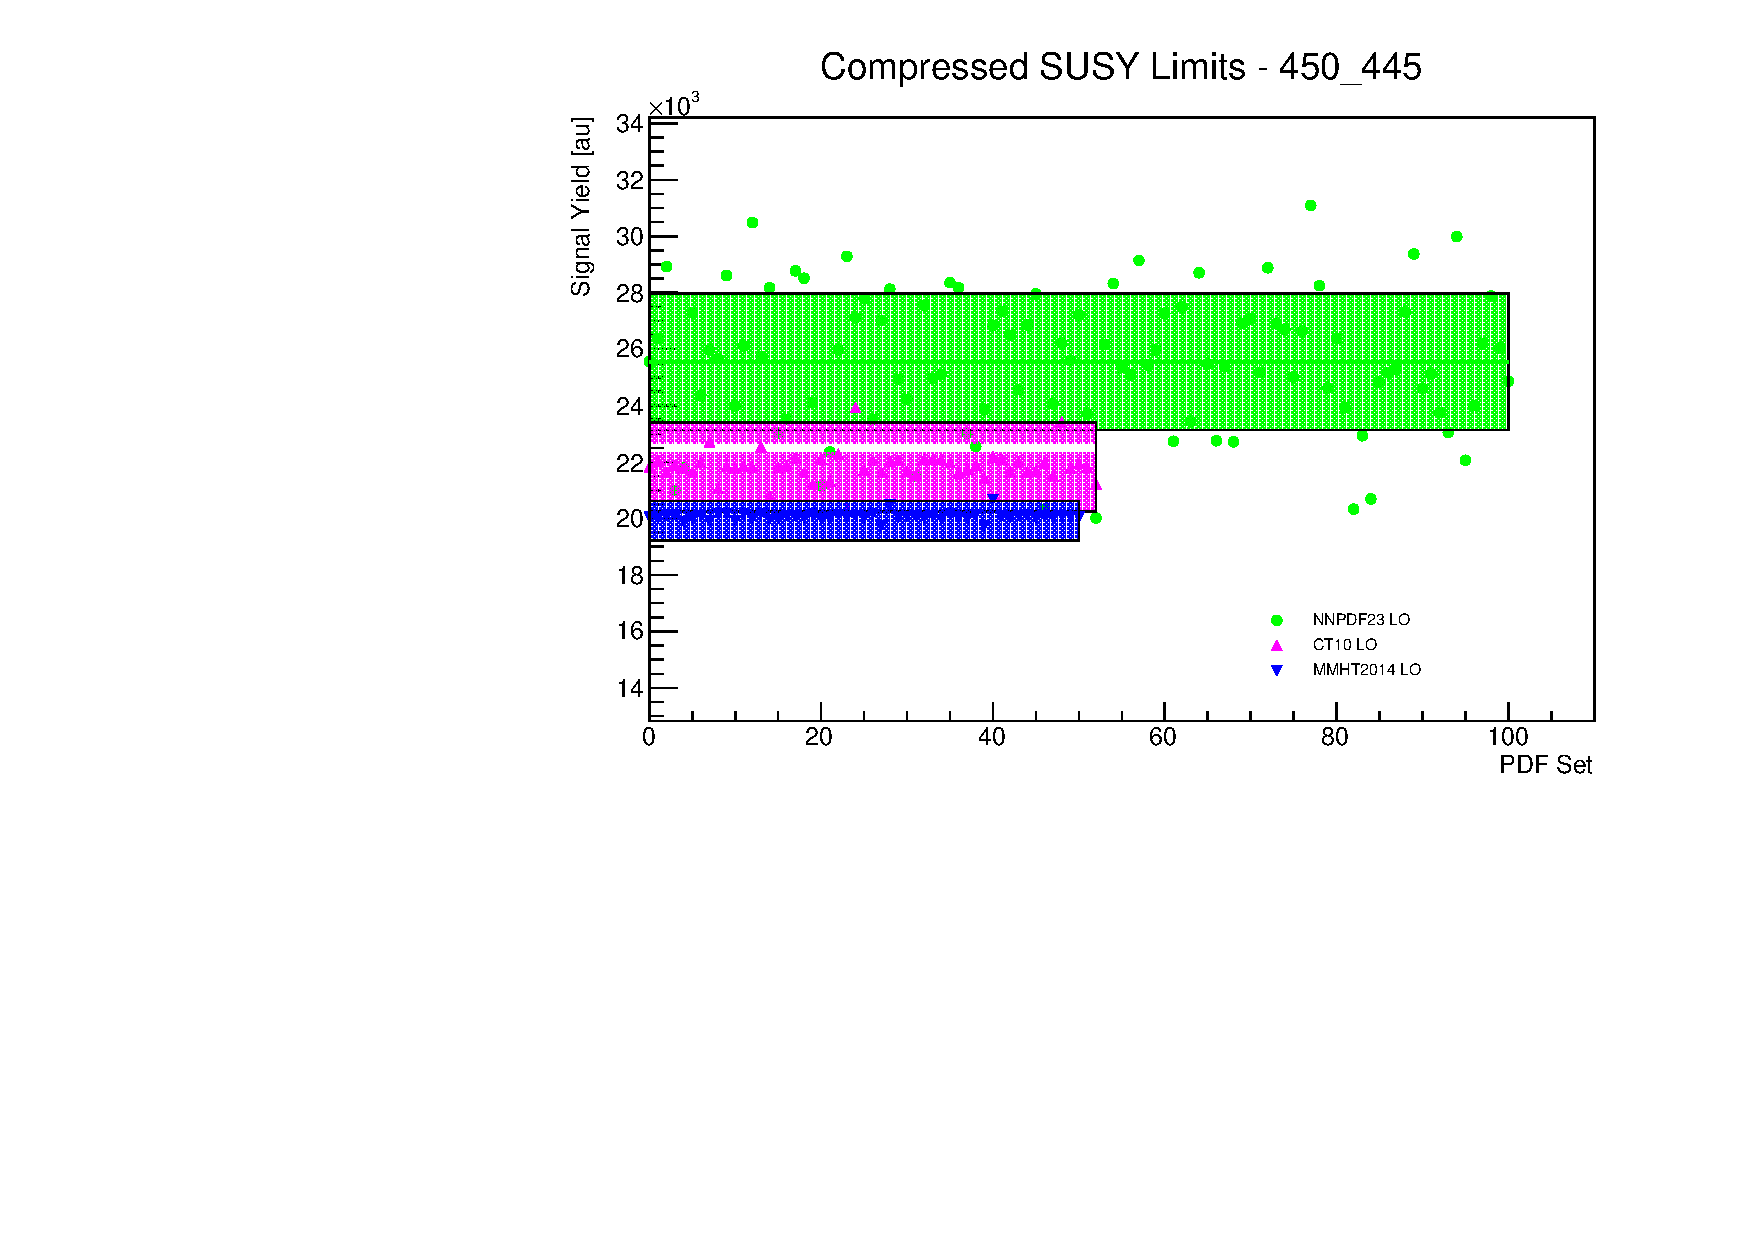
\includegraphics[width=\linewidth]{450_445_MCut0_pdfset}
\caption{Variation in \gls{susy} compressed weighted event yields for a model
  with $\msquark = 450$~GeV and $\mneutralino = 445$~GeV in the first $\met$ bin
  of the signal region ($250 < \met < 300$~GeV) for three \gls{pdf} sets NNPDF,
  CT10 and MMHT. The $x$-axis represents the different systematic uncertainties
  associated to each \gls{pdf} set.}
\label{fig:susy_pdfsysts}
\end{figure}

The \gls{pdf} uncertainties affects both the overall \gls{add} signal
normalization or cross section and the signal acceptance (the potential number
of events registered by the detector for a generated signal). These
uncertainties are collected in \cref{tab:susy_pdfsysts}. The increase of the
uncertainty on the cross section with the mass of the squark is due to the
higher momentum fraction of the partons required for its production. At these
energy regimes the \glspl{pdf} are less well known due to the lack of data to
extract the information from. A similar behavior is seen for the acceptance at
higher $\met$ values, also in this case there is a bias towards higher momentum
fraction of the partons involved in the production of the squark and thus to
region where the knowledge of the \glspl{pdf} is less precise. At low squark
masses and in the low $\met$ bin the statistics the systematic error increases
due to low Monte Carlo statistics.
\begin{table}
\centering
\small
\resizebox{\linewidth}{!}{\begin{tabular}{lccccccc}
  \toprule
  \multicolumn{8}{c}{\gls{pdf} Uncertainty} \\
  \midrule \midrule
  $\msquark$, $\mneutralino$ [GeV] &  400, 395 &
  450, 445 &  500, 495 &  550, 545 &  600, 595 &  650, 645 &  700, 695 \\
  \midrule
  $\Delta \sigma$  & 19 & 20 & 21 & 22 & 24 & 25 & 26 \\
  \midrule
  $\Delta A$ (250 $< \met <$ 300)  & 25 & 26 & 7 & 6 & 7 & 5 & 7\\
  $\Delta A$ (300 $< \met <$ 350)  & 5 & 7 & 5 & 4 & 4 & 4 & 4\\
  $\Delta A$ (350 $< \met <$ 400)  & 4 & 4 & 5 & 9 & 3 & 6 & 2\\
  $\Delta A$ (400 $< \met <$ 500)  & 6 & 2 & 6 & 5 & 2 & 7 & 9\\
  $\Delta A$ (500 $< \met <$ 600)  & 7 & 9 & 9 & 10 & 10 & 8 & 10\\
  $\Delta A$ (600 $< \met <$ 700)  & 8 & 10 & 6 & 14 & 13 & 10 & 9\\
  $\Delta A$ (700 $> \met$ )       & 10 & 9 & 16 & 15 & 17 & 16 & 14\\
  \bottomrule
\end{tabular}}
\caption{\gls{pdf} systematic uncertainties in \% on the SUSY compressed
  models. The uncertainty is the envelop that contains the signal yields from
  the three \gls{pdf} families, and their error bands. The first row indicates
  the systematic uncertainty on the overall normalisation. The following rows
  show uncertainty on the acceptance in the signal region $\met$ bins.}
\label{tab:susy_pdfsysts}
\end{table}
% The default \gls{pdf} for the event generation is NNPDF2.3. The PDF
% uncertainties are obtained by computing reweighting the signal samples to any of
% the following three PDF sets: NNPDF2.3LO, CT10LO and MMH2014LO and also varying
% each PDF set by its own uncertainties. This results in a large number of values
% for the signal event yield in the signal
% region. \cref{fig:susy_pdfsysts} shows an example of the observed
% variation in the event yield (y-axis) for the three PDF sets, each systematic
% variation of each PDF set is represented by a different position on the the
% x-axis. The PDF systematic uncertainty is decomposed in:
% \begin{itemize}
% \item An uncertainty $\Delta \sigma$ on the overall normalisation or cross
%   section, given by the variation of the total number of signal events,
% \item An uncertainty $\Delta A$ on the signal acceptance, which is defined by
%   the ratio of number of signal events in a particular bin of the signal region,
%   divided by the total number of signal events.
% \end{itemize}
% This decomposition is done since the ATLAS standard is to depict the uncertainty
% on the overall normalization as an uncertainty on the expected limits, while the
% uncertainty on acceptance is to be incorporated in the uncertainty on the
% observed limits. \cref{tab:susy_pdfsysts} presents the relative PDF uncertainty
% on $\Delta \sigma$ and $\Delta A$ in the different bins of the signal region,
% for each of the squark masses considered in the analysis. The uncertainty on the
% cross section is between 19 and 26\%, increasing at higher squark mass. The
% uncertainty on the acceptance increases for higher squark masses and at higher
% $\met$ bins. At low squark mass and in the low $\met$ bin the statistics is
% reduced and the systematic error increases due to low Monte Carlo statistics.
%%% Local Variables:
%%% mode: latex
%%% TeX-master: "../search_for_DM_LED_with_ATLAS"
%%% End:
